\documentclass[notes,blue,mathserif]{beamer}

\usepackage[latin1]{inputenc}
\usepackage[brazil]{babel}
\usepackage{graphicx}
\usepackage{fancybox}
%\usepackage{hyperref}


\usetheme{Boadilla}

% The default font theme installs a sans serif for all text of the presentation
%\usefonttheme{default}

% Using default block style
%\setbeamertemplate{blocks}[default]

% Background colors
% solid style
%\beamertemplatesolidbackgroundcolor{gray}
% gradient style
%\beamertemplateshadingbackground{blue!5}{yellow!10}
%\beamertemplateshadingbackground{blue!10}{yellow!5}
\beamertemplateshadingbackground{yellow!15}{blue!5}
%\beamertemplateshadingbackground{yellow!5}{blue!10}
% grid style
\beamertemplategridbackground[0.8in]

%Código para exibir layout antes de cada seção
%\AtBeginSubsection[]
\AtBeginSection[]
{
  \begin{frame}<beamer>
    \frametitle{Agenda}
%    \tableofcontents[currentsection,currentsubsection]
     \tableofcontents[currentsection]
  \end{frame}
}


\title[SMS Seguro]{Sistema de SMS Seguro\\PCS2050 - Projeto de Formatura II \\ Apresenta\c{c}\~{a}o Final}

\author[Cruz, Pereira, Silva]{Eduardo de Souza Cruz\\
					Geovandro Carlos Crepaldi Firmino Pereira\\
					Rodrigo Rodrigues da Silva\\ 
					Orientador: Prof. Dr. Paulo S. L. M. Barreto}
\institute[PCS/EPUSP]{Departamento de Engenharia de Computa\c{c}\~{a}o e Sistemas Digitais \\ Escola Polit\'{e}cnica da Universidade de S\~{a}o Paulo}
\date{S\~{a}o Paulo, 09/12/2008}

\begin{document}

\begin{frame}
\titlepage
\end{frame}


\section{Introdu\c{c}\~{a}o}

%%\subsection{Motiva\c{c}\~{a}o e Cen\'{a}rio}

\begin{frame}{Motiva\c{c}\~{a}o e Cen\'{a}rio}
\begin{itemize}[<+->]
\item Crescimento do uso do SMS no mundo: 
\begin{description}
\item 2,3 trilh\~{o}es de mensagens em 2010 (previs\~{a}o)
\end{description}
\item Plataforma leve e barata, com grande base de usu\'{a}rios:
\begin{description}
\item[]2,4 bilh\~{o}es de pessoas
\end{description}
\item Diversas oportunidades econ\^{o}micas: 
\begin{description}
\item72,5 bilh\~{o}es de d\'{o}lares para operadoras em 2006
\end{description}
\item Aus\^{e}ncia de uma solu\c{c}\~{a}o universalmente adotada.
\item Possibilidade de produzir pesquisa: inova\c{c}\~{a}o
\end{itemize}
\end{frame}

%%\subsection{Objetivos}

\begin{frame}{Objetivo}
\begin{block}

"Projetar, implementar e implantar um sistema capaz de prover confidencialidade, integridade e autenticidade ao servi\c{c}o de \emph{SMS} sem extrapolar as limita\c{c}\~{o}es de recursos t\'{i}picas do ambiente."
\end{block}
\end{frame}

%%\subsection{Metodologia}

\begin{frame}{Metodologia}
\begin{itemize}[<+->]
\item Estudo do cen\'{a}rio, detalhamento do problema e levantamento de requisitos
\item Estudo de esquemas de seguran\c{c}a em busca de uma solu\c{c}\~{a}o adequada ao problema
\item Projeto, implementa\c{c}\~{a}o e testes
\end{itemize}
\end{frame}

\section{Necessidade}

%\subsection{Aplica\c{c}\~{o}es Potenciais}

\begin{frame}{Aplica\c{c}\~{o}es Potenciais}
\begin{itemize}[<+->]
\item Comunica\c{c}\~{a}o interpessoal
\item Transa\c{c}\~{o}es banc\'{a}rias e pagamentos
\item Comunica\c{c}\~{a}o corporativa e governamental sigilosa
\item Monitora\c{c}\~{a}o remota
\end{itemize}
\end{frame}

%\subsection{Servi\c{c}os de Seguran\c{c}a}

\begin{frame}{Servi\c{c}os de Seguran\c{c}a}
\begin{itemize}[<+->]
\item Confidencialidade
\item Integridade
\item Autenticidade
\item Irretratabilidade
\end{itemize}
\end{frame}

%\subsection{Defini\c{c}\~{a}o do Problema}

\begin{frame}{Defini\c{c}\~{a}o do Problema}
\begin{itemize}[<+->]
\item SMS armazenado em aberto nas integradoras\/ e operadoras
\item Recursos limitados: processamento, mem\'{o}ria, largura de banda
\item Algoritmo \emph{A5} da rede \emph{GSM} quebrado
\item Poucas solu\c{c}\~{o}es de seguran\c{c}a no mercado
\item \emph{RSA}: cerca de \textit{20 mensagens} para trocar \textit{um} certificado
\item Algoritmos sim\'{e}tricos: Dificuldade em gerenciar as chaves
\end{itemize}
\end{frame}

%\subsection{M\'{e}tricas e Requisitos}

\begin{frame}{M\'{e}tricas e Requisitos}
\begin{itemize}[<+->]
\item Tempo de espera
\item Espa\c{c}o \'{u}til da mensagem
\item Tamanho da chave
\item \textit{Overhead} do protocolo
\end{itemize}
\end{frame}

\section{Solu\c{c}\~{a}o}

%\subsection{Especifica\c{c}\~{a}o}
\begin{frame}{Esquema de seguran�a desenvolvido}

Ao longo do trabalho, foi bolado um esquema de seguran�a inovador

\begin{itemize}[<+->]
\item Curvas el\'{i}pticas
\item Chaves menores
\item Criptografia auto-certificada
\item Criptografia baseada em identidades
\item Gerenciamento de chaves simplificado
\item Publica��o de artigo no SBSEG'08 definindo o novo esquema
\item Publica��o de artigo no WTICG'08 sobre o nosso projeto de formatura (men��o honrosa)
\end{itemize}

\end{frame}

%\subsection{Arquitetura}
\begin{frame}{Arquitetura}

%TODO: colar o diag de arquitetura
\end{frame}

\section{Implementa��o}

\begin{frame}{Implementa��o}
\begin{itemize}[<+->]
\item Esquema implementado em J2ME
\item Testes de viabilidade: OK
\item Implementa��o de protocolo de mensagens
\item Implementa��o de persist�ncia: Floggy
\end{itemize}
\end{frame}

\begin{frame}{Classes}


\begin{figure}
	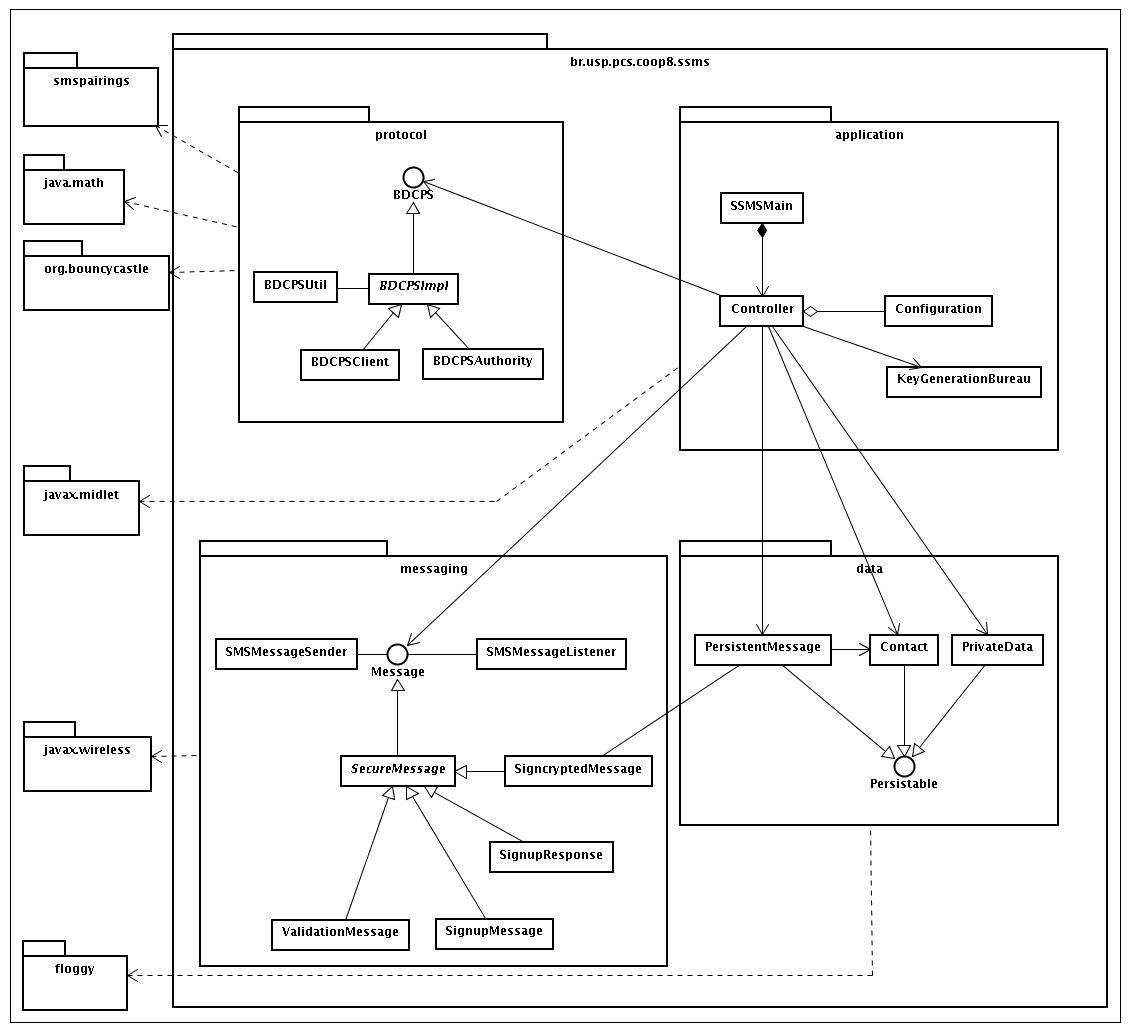
\includegraphics[width=0.65\textwidth]{figuras/class_diagram.PNG}
	\caption{Diagrama de classes do sistema}
\end{figure}

\end{frame}

%\subsection{Resultados}
\begin{frame}{Resultados}

\begin{table}[h]\centering
\caption{Testes com a implementa��o final (chaves de 176 bits)} \label{tab:bdcps176final}
\begin{tabular}{cccccc}\hline
Opera��o                   & Nokia E51(ms)   &  Nokia 6275(ms) & Emulador(ms)\\\hline
Set-Public-Value	&	66,9	& 750,6  & 204,5	 \\\hline
Private-Key-Extract &	379,0 &	4381,7 &	1033,9 \\\hline
Check-Private-Key	& 1164,9	& 12171,1  & 3209,9	 \\\hline
Set-Public-Key	& 379,5 &	4332,4 &	1013,3 \\\hline
Public-Key-Validate	&	1192,6 &	13112,0 & 3455,8 \\\hline
Signcryption	&302,4 &	1633,5 & 	428,8 \\\hline
Unsigncryption	&	266,7 &	1957,0 & 492,2 \\\hline
\end{tabular}
\end{table}
\end{frame}


\section{Conclus\~{a}o}

\begin{frame}{Conclus\~{a}o}

\begin{itemize}[<+->]
\item Projeto motivou a cria��o de um esquema criptogr�fico inovador
\item Solu��o implementada com sucesso, alta portabilidade
%TODO: algu�m p�e mais
\end{itemize}

\end{frame}

%??? adeus
%\subsection{Aplica\c{c}\~{a}o}
%\begin{frame}
%aplic
%\end{frame}

\begin{frame}{Contato}

	\begin{exampleblock}{Site do projeto}
		\begin{center}
		\begin{large}

		\textbf{http://secure-sms.googlecode.com}

		\end{large}
		\end{center}
	\end{exampleblock}

	\begin{exampleblock}{E-mail}
		\begin{center}
		\begin{large}

		\textbf{secure-sms@googlegroups.com}

		\end{large}
		\end{center}
	\end{exampleblock}

\end{frame}



\end{document}